% !TEX encoding = UTF-8 Unicode
\chapter{Twitter security methods}
Twitter, l'un des plus importants fournisseurs d'API multimédia, qui compte 307 millions de clients actifs par mois \cite{17}, fournit diverses méthodes pour récupérer ses données au nom de l'utilisateur de Twitter en utilisant son application. En faisant des appels autorisés aux API de Twitter, l'application peut accéder aux amis et aux adeptes de n'importe quel compte, récupérer toute information d'utilisateur et accéder aux ressources de l'utilisateur. Par cette commodité, une énorme quantité de sites Web intégrés utilisent Twitter API REST chaque jour et cette tendance n'a pas de fin au moins pour les prochaines années. Cependant, cela conduirait à un grand risque et un défi pour Twitter de sécuriser ses références client. Ce chapitre analyse et se concentre sur la façon dont Twitter autorise ces applications pour éviter la fuite des ressources de l'utilisateur de façon inattendue.
\section{Résumé de la méthode de sécurité twitter : 3-Legged Oauth 2.0}
Twitter vérifie les droit de l'application en suivant le modèle OAuth 2.0 à 3 pattes. Ce modèle est l'interaction entre trois rôles, c'est pourquoi ce modèle a nommé OAuth à trois pattes, le propriétaire de la ressource, le serveur et le client (application). Le flux global de ce modèle est que le propriétaire de la ressource doit accorder l'accès et restreindre l'interaction au client et ce dernier communique avec le serveur par le jeton d'accès au nom de ce propriétaire de ressource. De cette façon, l'application est capable de récupérer ce que l'utilisateur à accés. Cela réduit le risque de perte et de modification des ressources. Pour envoyer une requête valide, l'application doit obtenir le jeton d'accès au nom d'un utilisateur de Twitter. Il s'agit de la phase obligatoire et de la première étape du processus d'authentification. Il vise à:
\begin{itemize}
\item Définir si l'application a les droits pour accéder à un compte d'utilisateur. L'utilisateur doit accorder l'accès à l'application à son compte manuellement pour récupérer des données. Cela prouve non seulement que l'utilisateur est au courant de l'existence de l'application, mais prend également en charge l'utilisateur pour gérer le droit d'application. Chaque fois que l'internaute se sent insatisfait de cette demande, il / elle est libre de bloquer l'accès à l'application.
\item Limiter l'interaction de l'application. L'application est uniquement en mesure de mettre en œuvre ce que les utilisateurs lui ont permis de faire. Cela signifie que l'application ne peut pas interagir sur les ressources auxquelles le propriétaire de la ressource n'accorde pas d'accès. Cela aide à protéger les ressources et à maintenir l'intégrité du système en évitant une fuite d'information ou un changement accidentel de la ressource.

\end{itemize}

\textit{S'authentifier avec Twitter.}


Twitter continue à demander de fournir un nom d'utilisateur valide et mot de passe, puis continuer avec le processus ci-dessus.
\begin{figure}[! ht ]
			\centering
			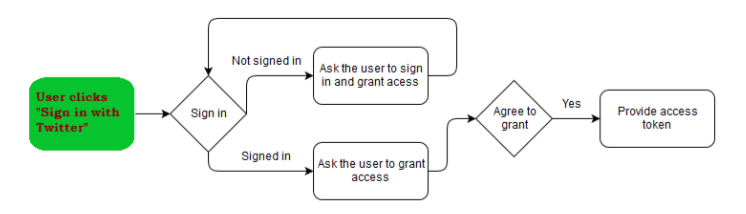
\includegraphics[scale=.4]{./images/twitter_signin.png}
			\caption {API growth}
		\end{figure}
		
Selon "OAuth FAQ" Document sur Twitter \cite{3}, actuellement Twitter n'expire pas le jeton d'accès. Cela signifie que le jeton d'accès sera valide tant que l'utilisateur autorise son accès. De mon point de vue, cela apporterait de nombreux avantages tant pour l'utilisateur que pour l'application. Tout d'abord, l'application n'est pas obligée d'envoyer une requête pour générer de nouveaux jetons d'accès fréquemment et, par conséquent, la charge de travail sur le serveur et le côté client sont considérablement réduites. Deuxièmement, le client n'est pas tenu de se connecter chaque fois que le jeton d'accès précédent soit expiré.

La mise en œuvre de Twitter, qui repose sur le flux de la spécification OAuth 2 de Grant (dans la section 3.2.1), est illustrée à la Figure 10. Prenons maintenant un aperçu du flux technique en détail pour voir comment Twitter authentifie le propriétaire de la ressource et Application pour générer un jeton d'accès.

Step 1: Obtaining a request token 

Au début, l'application doit envoyer la requête au serveur OAuth pour générer un jeton de demande. Ce jeton est représenté pour un client spécifique et ce n'est pas un jeton d'accès, ce qui signifie que ce propriétaire de ressource doit accorder l'accès à l'application à travers ce jeton de demande.
\begin{figure}[! ht ]
			\centering
			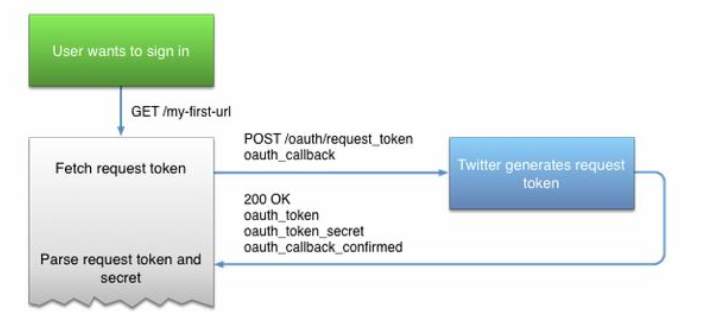
\includegraphics[scale=.4]{./images/twitter_token_generation.png}
			\caption {API growth}
		\end{figure}
		
La figure 10 montre le flux global pour cette étape, l'application doit envoyer la requête POST incluant ses informations d'identification au serveur. Après cela, Twitter génère le jeton de demande et le renvoie. Voici un exemple de la demande:

%%code goes here %%%

\begin{verbatim}
POST /oauth/request_token HTTP/1.1
User-Agent: themattharris' HTTP Client
Host: api.twitter.com
 Accept: */*
Authorization:
               OAuth oauth_callback="http%3A%2F%2Flocalhost%2Fsign-in-
with-twitter%2F", oauth_consumer_key="cChZNFj6T5R0TigYB9yd1w",
                      oauth_nonce="ea9ec8429b68d6b77cd5600adbbb0456", 
                       oauth_signature="F1Li3tvehgcraF8DMJ7OyxO4w9Y%3D", 
                       oauth_signature_method="HMAC-SHA1",                            
                      oauth_timestamp="1318467427",
                      oauth_version="1.0"
\end{verbatim}


Il y a deux arguments les plus importants dans cette demande. Elles sont:
\begin{itemize}
\item Oauth\_consumer\_key: La valeur représente le client (application). Cette valeur a pour but de notifier au serveur d'authentification quel client demande le jeton de demande et d'éviter toute erreur dans la relation de mappage entre le client et le propriétaire de la ressource.
\item Oauth\_callback: Il s'agit d'un lien vers lequel le serveur d'authentification va naviguer après sa connexion réussie. Twitter inclura le jeton d'accès et jeton secret dans la réponse et les renvoie à l'application à ce lien. Par conséquent, à cette étape, l'application doit avertir le serveur de la destination de ces informations top-secret pour éviter la fuite des informations d'identification sensibles.
\end{itemize}

step 2 : Redirecting the user

Après la première étape, le serveur d'authentification est informé par le client du propriétaire de la ressource qui souhaite autoriser l'accès à cette application. Ainsi, à cette étape, le client doit naviguer entre le propriétaire de la ressource et le serveur afin de vérifier lui-même et d'accorder l'accès comme le montre la Figure 11.
\begin{figure}[! ht ]
			\centering
			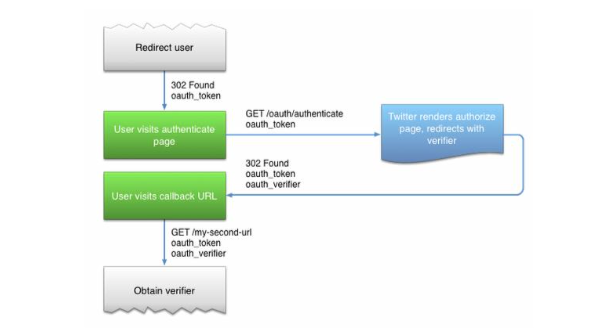
\includegraphics[scale=.4]{./images/twitter_redirecting_user.png}
			\caption {API growth}
		\end{figure}

Tout d'abord, le client doit inclure le jeton de demande qui est retourné par le serveur à l'étape 1 et parcourir sa ressource à la page d'authentification (page de connexion) en utilisant la redirection HTTP 302. Ensuite, le propriétaire de la ressource doit fournir un nom d'utilisateur et un mot de passe valides. Selon le statut du propriétaire de la ressource, il y a trois cas possibles:
\begin{itemize}
\item Signé et approuvé. Si le propriétaire de la ressource a déjà accepté et approuvé l'application, cette étape sera ignorée et le serveur renverra automatiquement le jeton d'accès valide à l'URL de rappel immédiatement.
\item Signé mais non approuvé. Si le propriétaire de la ressource a signé, cependant, il n'a pas approuvé l'application encore (comme mentionné ci-dessus, le propriétaire de la ressource se doit d'approuver le client qu'une seule fois), l'authentification est affichée pour l'utilisateur pour accorder et gérer l'accès de l'application. Après cela, le jeton de demande sera retourné.
\item Non connecté. Pour le nouveau propriétaire de la ressource qui n'a pas signé et approuvé l'application, la page de connexion s'affiche afin d'entrer le nom d'utilisateur et le mot de passe. Ensuite, le flux sera identique à l'état "Signé mais non approuvé".
\end{itemize}
Voici les pages d'authentification : 

step 3 :  Converting the request token to an access token

Après l'étape 2, le propriétaire de la ressource a déjà publié le droit à l'application. En ce moment, l'application est en mesure d'accéder aux ressources et de récupérer des données, cependant, il ya une étape de plus à terminer. Il obtient le jeton d'accès en validant le jeton de demande. Cette étape vise à informer le serveur que le propriétaire de la ressource a autorisé l'accès de l'application.

Voici l'exemple de demande de jeton d'accès:

\begin{verbatim}
POST /oauth/access_token HTTP/1.1
User-Agent: themattharris' HTTP Client
Host: api.twitter.com
Accept: */*
Authorization: OAuth oauth_consumer_key="cChZNFj6T5R0TigYB9yd1w",    
                       oauth_nonce="a9900fe68e2573b27a37f10fbad6a755",  
                       oauth_signature="39cipBtIOHEEnybAR4sATQTpl2I%3D", 
                       oauth_signature_method="HMAC-SHA1", oauth_timestamp="1318467427",
                       oauth_version="1.0", 
                       
oauth_token="NPcudxy0yU5T3tBzho7iCotZ3cnetKwcTIRlX0”
Content-Length: 57
Content-Type: application/x-www-form-urlencoded
oauth_verifier=uw7NjWHT6OJ1MpJOXsHfNxoAhPKpgI8BlYDhxEjIBY
\end{verbatim}

L'application doit envoyer une requête POST au serveur d'authentification pour mettre à niveau le jeton de demande. Dans cette demande, deux arguments qui une fois de plus illustrer la haute sécurité de la mise en œuvre Twitter:
\begin{itemize}
\item Oauth\_token: Le jeton de demande qui a été retourné à l'étape 1. L'application doit clarifier quel jeton utiliser pour communiquer avec le serveur pour le compte du propriétaire de la ressource. Toutefois, si une autre application falsifie le jeton de demande et l'envoie au serveur au nom de l'application, si le serveur ne vérifie pas la validité de ce jeton de demande et renvoie le jeton d'accès valide à l'application sophistiquée. Par coïncidence, le serveur d'authentification révèle juste ses informations d'identification utilisateur . C'est la raison pour laquelle chaque demande doit inclure le deuxième argument.
\item Oauth\_verifier: Il s'agit de la valeur renvoyée est l'étape 2. Cette valeur a pour but de notifier au serveur la validité du jeton de demande. Cette valeur ne sera retournée que lorsque le propriétaire de la ressource aura accepté l'application. Le vérificateur oauth dans la requête doit correspondre au vérificateur oauth qui a été stocké dans le serveur après l'étape 2. Par conséquent, la requête sophistiquée ne peut pas être autorisée sans un auth\_verifier valide.
\end{itemize}
Après avoir récupéré le jeton d'accès, le client peut communiquer avec le serveur par ce jeton au nom du propriétaire de la ressource pour collecter des données, créer un objet et même supprimer la ressource si possible tant que le propriétaire de la ressource a accepté ce client.

En général, l'implémentation Twitter sur l'authentification de l'application a été analysée. Actuellement, Twitter applique 3-Legged OAuth 2.0 qui représente le propriétaire de ressource, le serveur et le client (application). Dans ce modèle, le propriétaire de la ressource doit se s'authentifier auprès du serveur en fournissant un nom d'utilisateur et un mot de passe valides. Après cela, il / elle doit habiliter l'application à interagir sur ses données. Enfin, le serveur émet un jeton d'accès à l'application et il peut être utilisé pour le compte du propriétaire de la ressource. Jusqu'à présent, nous avons clarifié la relation, les dépendances entre le propriétaire de la ressource, le serveur et l'application. Dans la section suivante, nous continuons à rechercher les conditions de communication entre l'application et le serveur.
		
\section{Authentication \& Authorization in Twitter API calls}
L'application peut envoyer de nombreuses requêtes à l'API de Twitter pour récupérer, supprimer et créer des ressources. D'une part, cela pourrait rapprocher Twitter du public en raison de l'énorme ressource d'information et de ses flexibilités. D'autre part, cela pourrait être le plus grand risque pour Twitter car il pourrait y avoir des millions de requêtes venant de millions d'application chaque jour. Par conséquent, il ya deux charges exceptionnelles auxquelles Twitter est confronté:
\begin{itemize}
\item Comment Twitter peut-il authentifier l'application et ses demandes?
\item Comment Twitter sécuriser l'information sensible, contenu dans les requêtes comme l'accès
Jeton, jeton d'accès secret, clé client et secret client?
\end{itemize}
La réponse clé a été introduite ci-dessus à la section 3.2.2. Twitter applique partiellement l'infrastructure à clé publique pour protéger les données sensibles envoyées entre le client et le serveur. Afin de tester cette fonction, nous allons rechercher quelles étapes sont nécessaires pour envoyer et lire la demande côté client et côté serveur, au cas où l'application envoie la requête de tweeter un nouveau tweet sur le serveur de Twitter:

Le coté client : 

Les données brutes ne sont pas censées être envoyées de client à serveur puisque l'autre application est capable d'écouter et de capturer ces secrets. Par conséquent, avant d'envoyer la requête, l'application doit nécessairement masquer la clarté du message en utilisant l'algorithme de hachage. Le flux global peut être expliqué par la figure 13.
\begin{figure}[! ht ]
			\centering
			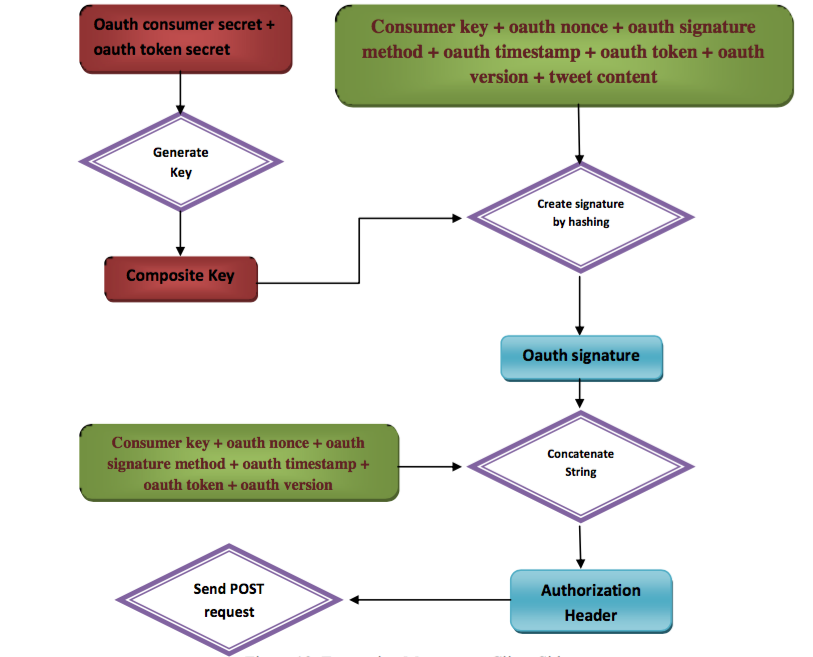
\includegraphics[scale=.4]{./images/twitter_client_side.png}
			\caption {API growth}
		\end{figure}
\newpage
		
Comme on peut le voir sur la figure ci-dessus, au début, l'application doit calculer une clé composite à partir de deux clés privées, le secret de consommateur OAuth et le secret de jeton OAuth. Ces deux clés sont censées être confidentielles. Ensuite, l'application doit créer la signature par hachage du message, qui est concacténée à partir de nombreux arguments tels que la clé de consommateur, oauth nonce, méthode de signature oauth, timestamp oauth, jeton oauth, version oauth et la valeur de la requête dans ce cas est le contenu tweet. Enfin, la signature oauth sera placée dans l'en-tête d'autorisation dans la requête POST HTTP avec d'autres arguments et envoyée au serveur Twitter. Voici l'exemple de la demande POST d'une application:

%%code goes here %%% 

\begin{verbatim}
POST 
/1.1/statuses/update.json?status=New%20Tweet%20from%20API&display_coordinates
=false HTTP/1.1

Authorization: OAuthoauth_consumer_key="DC0sePOBbQ8bYdC8r4Smg" 
                      oauth_signature_method="HMACSHA1"
                      oauth_timestamp="1447763195" oauth_nonce="2757352841" 
                      oauth_version="1.0" 
                      oauth_token="4204335839-
JKlJnO249TnMegiDsJaqDkxgDyDPizQQIi8nVO7" 
                      oauth_signature="zkKRtFwatfH8qjn%2FvxQnhnhyowY%3D"
Host: api.twitter.com
\end{verbatim}


Il semble y avoir quelques arguments dupliqués dans ce processus tels que la clé de consommateur, oauth nonce, méthode de signature oauth et ainsi de suite. Cependant, dans la section 2.2.4 selon les apatrides, toutes les informations essentielles pour cette demande doivent être incluses dans la demande. Par conséquent, chaque argument joue un rôle différent dans le décryptage et le processus d'authentification tels que:

\begin{itemize}
\item Oauth\_consumer\_key: notifie au serveur quelle application envoie un appel API.
\item Oauth\_signature\_method: algorithme de hachage qui a été appliqué pour calculer la signature. L'authentification doit connaître cette méthode puisque le serveur va calculer la signature une fois de plus par elle-même pour valider la signature.
\item Oauth\_timestamp, oauth\_nonce, oauth\_version: Ces trois arguments ont été utilisés pour générer la signature, ainsi, le serveur doit les collecter. En outre, comme mentionné ci-dessus, ces arguments aident à empêcher l'attaque de texte en clair.
\item Oauth\_token: le jeton valide qui représente pour le droit de l'application. Le serveur d'authentification qualifie les appels API de l'application par ce jeton.
\item Oauth\_signature: le message chiffré du client. Ce message illustre ce que l'application souhaite que le serveur de ressources implémente.
\end{itemize}
Dans ce cas, Twitter applique le modèle PKI, donc, il ya une paire de clés qui utilise le processus d'authentification. Malgré le nom différent, la clé (clé publique) et le secret (la clé privée), ils jouent toujours le même rôle. Cependant, il ya un changement majeur dans le processus de cryptage. Au lieu de crypter le message entier, Twitter requiert seulement que le message soit haché en utilisant l'algorithme HMACSHA1 en utilisant la clé qui a été calculée à partir de deux clés secrètes. Les principaux objectifs de cette étape sont les suivants:
\begin{itemize}
\item Cacher l'explicité du message. Évidemment, envoyer les informations brutes entre serveur et client n'est jamais une bonne solution puisque le pirate peut écouter votre appel, ainsi, Twitter demande à l'application de crypter ces informations confidentielles par des clés secrètes.
\item Adresser la validité de la demande. Comme on peut le voir sur l'extrait de code 3, certains arguments tels que oauth\_token, oauth\_consumer\_key sont transmis directement et envoyés directement au serveur sans cryptage. Par conséquent, la signature joue un rôle comme la certification pour la demande valide. Étant donné que la signature a été calculée par les deux clés secrètes, bien que l'oauth\_token, oauth\_consumer\_key soient distribués communément, l'autre application ne peut pas falsifier la requête sans la signature valide. Pour cette raison, les autres arguments ne sont pas chiffrés et transparents.
\end{itemize}

Le coté serveur : 

Selon les règles du modèle PKI, après avoir reçu la demande de l'application, le serveur va valider la demande en comparant deux valeurs de la signature. Le premier est la signature originale dans la requête et le second est le résultat après le calcul de la signature par le serveur. Cette section explique comment le serveur calcule la signature par lui-même. Cette section réutilisera l'extrait de code 3 comme exemple.


\begin{verbatim}

POST 
/1.1/statuses/update.json?status=New%20Tweet%20from%20API&display_coordinates
 =false
\end{verbatim}


%%code goes here %%%% 

Comme défini dans la section 2.2.2, le serveur sépare la valeur de la requête de l'URL. Dans ce cas, la valeur est le contenu du nouveau tweet et il est "New Tweet from API". Retour à Figure 13, afin de générer la signature, le serveur prendra le contenu tweet de l'URL et les autres arguments dans la demande. A ce stade, le serveur calcule la clé à partir de deux clés secrètes basées sur la clé oauth\_consumer\_key et la oauth\_token dans la requête. Le point intéressant est que serveur Twitter enregistre toutes les clés publiques et privées de toutes les applications, ainsi, le serveur est capable de calculer la clé sans demander ces clés secrètes de client. Enfin, le serveur compare la signature de la requête et la signature qui a été générée par elle-même. Si les deux signatures sont identiques, le serveur exécutera automatiquement cette requête et répondra à la requête du client, sinon le serveur ne suivra pas cette requête et renverra un message d'erreur.

Le processus d'authentification côté serveur vise à:
\begin{itemize}
\item Prouver la validité de la demande. En testant la signature, le serveur est en mesure de vérifier la demande envoyée par l'application autorisée.
\item Vérifiez le droit de l'application. Grâce à la méthode HTTP et au message, le serveur peut vérifier si l'application est autorisée à déclencher cette requête. Si l'application n'a pas encore accordé l'accès, le serveur retournera un message d'erreur sans exécuter cette requête.
\item Vérifiez la fiabilité du message. Le serveur doit vérifier le message pour s'assurer qu'il est le message original du client sans aucune modification ou changement par un tiers. Hash est un chiffrement unidirectionnel et dans ce cas, le message a été haché en utilisant les deux clés secrètes, donc, il est presque impossible pour une autre application de fausser la signature et le message en même temps. Dans le cas où le message a été falsifié, lorsque le serveur calcule la signature et compare deux valeurs, ces deux valeurs ne peuvent pas être identiques et cette requête se révèle invalide.
\end{itemize}
Dans l'ensemble, afin de protéger le propriétaire de la ressource, Twitter s'attend à ce que leurs clients émettent le droit à l'application en utilisant l'authentification à 3 jambes. Après cela, l'application passe le jeton, qui est représenté pour son droit, à la requête et communique avec le serveur par ce jeton. L'application est capable de travailler sur les ressources sur lesquelles le propriétaire de la ressource lui permettrait d'interagir. Afin de sécuriser les informations sensibles qui sont envoyées d'avant en arrière entre le client et le serveur, l'application doit générer la signature à partir du message en le hachant avec deux clés secrètes. La valeur évidente du message ne doit pas être envoyée directement au serveur pour éviter la fuite des informations top secret.

Dans le chapitre suivant, la fonction de sécurité d'un fournisseur d'API sera exécutée. Prenons un autre regard sur la façon dont les détails de l'utilisateur, tels que le numéro de compte bancaire et de sécurité, sont protégés lors de transactions. Le prochain chapitre utilisera le Stripe, un fournisseur de paiement en ligne, et ses services comme exemple.


		
		
















		